% !TeX root = RJwrapper.tex

\renewcommand{\labelenumii}{\arabic{enumi}-\arabic{enumii}}
\renewcommand{\arraystretch}{1.3}

\title{boinet: An R Package for Bayesian Optimal Interval Design for Dose Finding Based on Both Efficacy and Toxicity Outcomes}
\author{by Yusuke Yamaguchi, Kentaro Takeda and Kazushi Maruo}

\maketitle

\begin{abstract}
Bayesian optimal interval based on both efficacy and toxicity outcomes (BOIN-ET) design is a model-assisted oncology phase I/II trial design, aiming to establish an optimal biological dose accounting for efficacy and toxicity in the framework of dose-finding. Some extensions of BOIN-ET design are also available to allow for time-to-event efficacy and toxicity outcomes based on cumulative and pending data (time-to-event BOIN-ET: TITE-BOIN-ET), ordinal graded efficacy and toxicity outcomes (generalized BOIN-ET: gBOIN-ET), and their combination (TITE-gBOIN-ET). \CRANpkg{boinet} package is an R package to implement the BOIN-ET design family. The package supports the conduct of simulation studies to assess operating characteristics of BOIN-ET, TITE-BOIN-ET, gBOIN-ET, and TITE-gBOIN-ET designs, where users can choose design parameters in flexible and straightforward ways depending on their own application. We demonstrate its capability and effectiveness using several simulation studies.
\end{abstract}

\section{Introduction}
A paradigm shift in anti-cancer treatment with the emergence of molecular targeted agents and immunotherapies is calling for a reform of dose-finding strategy in phase I oncology clinical trials. Traditional dose-finding procedures designed to establish the maximum tolerated dose underlie an assumption of a monotonic dose-efficacy relationship; that is, the higher dose level is assumed to be more toxic and efficacious. However, the monotonic dose-efficacy relationship would be doubtful in many cases of the targeted agents and immunotherapies, where the efficacy may reach a plateau beyond a given dose level or even take an umbrella shape \citep{calabrese:2001,lorusso:2010,reynolds:2010}. Accordingly, a concept of optimal biological dose (OBD) has been introduced into the framework of dose-finding \citep{corbaux:2019,fraisse:2021}. The OBD, which is generally defined as a tolerable dose having adequate efficacy under an assumption of non-monotonic dose-efficacy relationships, is established with a dose-escalation rule based jointly on toxicity and efficacy. Numerous dose-finding designs to incorporate the trade-off between toxicity and efficacy have been proposed, broadly classified as algorithm-based designs \citep{lin:2020a}, model-based designs \citep{thall:2004,yuan:2016,riviere:2018}, and model-assisted designs \citep{takeda:2018,yuan:2019,li:2020,lin:2020b,yin:2020,lin:2021}. Particularly, the model-assisted designs are known to yield superior performance compared with more complicated model-based designs and to be implemented in as simple a way as the algorithm-based designs \citep{yuan:2019}.

Bayesian optimal interval based on efficacy and toxicity outcomes (BOIN-ET) design proposed by \citet{takeda:2018} is one of the model-assisted designs and has been widely used to establish the OBD, where the dose-escalation decision is determined by minimizing a posterior probability of incorrect dose assignments in terms of both efficacy and toxicity. Furthermore, the BOIN-ET design has been extended in two ways to accommodate important clinical features unique to molecular targeted agents and immunotherapies. Firstly, the occurrence of efficacy responses and/or adverse events may be delayed due to the mechanism of the agents. Such late-onset efficacy and toxicity outcomes usually require a longer assessment window than the typical first one or two cycles for the traditional cytotoxic agents \citep{postel:2009,weber:2015}. Ignoring the feature of late-onset toxicity may cause potential dose reductions or interruptions in later phase trials. To allow for sequential enrollment even before patients have completed the required efficacy and toxicity assessment window, \citet{takeda:2020} proposed time-to-event BOIN-ET (TITE-BOIN-ET) design, which extends the BOIN-ET design to use cumulative and pending data of both efficacy and toxicity for the dose-escalation decision \citep{lin:2020c}. Secondly, the efficacy and toxicity outcomes are often summarized by binary outcomes, scored as an overall response (ORR) or not an ORR for efficacy, and scored as a dose-limiting toxicity (DLT) or not a DLT for toxicity; however, the molecular targeted agents and immunotherapies are more likely to be featured by multiple low or moderate grades of toxicities than DLTs \citep{penel:2011}. Besides, the efficacy response may prefer to be evaluated by the combination of ORR and long-term stable disease (SD) in solid tumors and by accounting for the difference between complete remission (CR) and partial remission (PR) in lymphoma. To allow for the ordinal graded efficacy and toxicity assessment, \citet{takeda:2022b} proposed generalized BOIN-ET (gBOIN-ET), which extends the BOIN-ET design to use ordinal graded efficacy and toxicity data for the dose-escalation decision. \citet{takeda:2023} proposed time-to-event generalized BOIN-ET (TITE-gBOIN-ET) to address simultaneously the aforementioned challenges of the late-onset ordinal graded efficacy and toxicity outcomes. \CRANpkg{Keyboard} package \citep{xiaomeng:2025} and \CRANpkg{escalation} package \citep{kristian:2024} are existing R packages that implement other types of the OBD-finding designs, while there are no R packages that provide functions to implement the BOIN-ET, TITE-BOIN-ET, gBOIN-ET, and TITE-gBOIN-ET design.

\CRANpkg{boinet} package \citep{yamaguchi:2025} is an R package to implement the BOIN-ET design family. The package supports the conduct of simulation studies to assess operating characteristics of BOIN-ET, TITE-BOIN-ET, gBOIN-ET, and TITE-gBOIN-ET, where users can choose design parameters in flexible and straightforward ways depending on their own application. It should be noted that the selection of OBD in the BOIN-ET design family is carried out at the end of the trial after completing the dose-escalation procedure: (i) the toxicity and efficacy probabilities at each dose level are estimated using all data obtained from the entire cohort, and then (ii) given the estimated toxicity and efficacy probabilities, the utility to measure the toxicity-efficacy trade-off is computed and serves as a basis for the OBD selection. The \CRANpkg{boinet} package offers several options regarding methods to estimate the efficacy probability and measures to select the OBD. The operating characteristics of the design are summarized by the percentage of times that each dose level is selected as OBD and the average number of patients who are treated at each dose level. The percentage of times that the study is terminated and the expected study duration are also provided. We demonstrate the capability and effectiveness of the \CRANpkg{boinet} package.

This article is organized as follows. We first describe the BOIN-ET, TITE-BOIN-ET, gBOIN-ET, and TITE-gBOIN-ET designs implemented by the package. We then provide details on how to use the \CRANpkg{boinet} package through simulation studies. The article is concluded with a brief discussion.

\section{Case example}
The BOIN-ET design family is a relatively new methodological development, and while they are being implemented in ongoing trials, published case results using these specific designs are still forthcoming. We here provide one case study that has actually implemented the TITE-BOIN-ET design.

A two-part phase I/II study evaluating a combination of luspatercept and erythropoiesis-stimulating agent (ESA) in patients with low-risk myelodysplastic syndromes without ring sideroblasts having failed to achieve a response after ESA without disease progression is being conducted \citep{ades:2024}. The primary objective of this dose-finding part of the trial was to determine the optimal dose in terms of both toxicity and efficacy for luspatercept + ESA, for selection in the randomized part B of the trial. Based on a TITE-BOIN-ET design, four dose levels were tested: Dose level 1 (n=3); Dose level 2 (n=3); Dose Level 3 (n=3); Dose Level 4 (n=15). The toxicity was measured by a dose-limiting toxicity at Day 21 of cycle 1 for non-hematological toxicity, up to Day 42 for hematological toxicity. The efficacy was measured by a response rate (complete response + partial response + stable disease with hematological improvement), and the assessment window for efficacy was 21 days.

\section{Methodology}
Consider a dose-finding trial aiming to determine the OBD of a test drug, and suppose that $J$ dose levels are investigated by sequentially assigning small cohorts of patients to the next dose levels until reaching a maximum number of patients enrolled. Suppose that patients in the current cohort have been treated at dose level $j$, and let $n_j$ denote the cumulative number of patients treated at dose level $j$ for $j=1,\ldots,J$. Let $\tau_T$ and $\tau_E$ be the assessment window for toxicity and efficacy respectively. We below describe the dose-escalation procedure in the BOIN-ET, TITE-BOIN-ET, gBOIN-ET, and TITE-gBOIN-ET designs, followed by an introduction to the OBD selection. Further details are found in the original articles \citep{takeda:2018,takeda:2020,takeda:2022a,takeda:2022b,takeda:2023}.

\subsection{Dose-escalation procedure in BOIN-ET and TITE-BOIN-ET design}
Let $p_{Tj}$ and $p_{Ej}$ be a true toxicity and efficacy probability at dose level $j$ for $ j=1,\ldots,J$, respectively. Let $\phi^p$ and $\delta^p$ be a target toxicity and efficacy probability respectively, which are pre-specified by trial physicians according to the disease and the definition of toxicity and efficacy. Lower and upper toxicity boundaries are pre-specified as $\lambda^p_1$ and $\lambda^p_2$ respectively, which satisfy a condition of $0\leq\lambda^p_1\leq\phi^p\leq\lambda^p_2<1$. A lower efficacy boundary is also pre-specified as $\eta^p_1$ with a condition of $0\leq\eta^p_1<\delta^p<1$. Let $\hat{p}_{Tj}$ and $\hat{p}_{Ej}$ be an observed toxicity and efficacy probability at dose level $j$ respectively, which are calculated using the cumulative toxicity and efficacy data in different ways for the BOIN-ET and TITE-BOIN-ET design (see subsections below). Then, the dose level used in the next cohort is determined by the following rule:
\begin{enumerate}
\item If $\hat{p}_{Tj}\leq\lambda^p_1$ and $\hat{p}_{Ej}\leq\eta^p_1$, escalate to dose level $j+1$.
\item If $\hat{p}_{Tj}<\lambda^p_2$ and $\hat{p}_{Ej}>\eta^p_1$, stay at the same dose level $j$.
\item If $\hat{p}_{Tj}\geq\lambda^p_2$, de-escalate to dose level $j-1$.
\item If $\lambda^p_1<\hat{p}_{Tj}<\lambda^p_2$ and $\hat{p}_{Ej}\leq\eta^p_1$, consider the following additional rules:
  \begin{enumerate}
  \item If dose level $j+1$ has never been used until the current cohort, escalate to dose level $j+1$. 
  \item Otherwise, choose $\arg\max_{j'\in\{j-1,j,j+1\}}\hat{p}_{Ej'}$ as the dose level for the next cohort; if more than two dose levels have the same highest observed efficacy probability, randomly select one of them. 
  \end{enumerate}
\end{enumerate}
Optimal values of $(\lambda^p_1,\lambda^p_2,\eta^p_1)$ are determined as values that minimize a posterior probability of incorrect decisions under the following six hypotheses:
\begin{gather*}
H_{1j}: (p_{Tj}=\phi^p_1,p_{Ej}=\delta^p_1),\quad H_{2j}: (p_{Tj}=\phi^p_1,p_{Ej}=\delta^p),\quad H_{3j}: (p_{Tj}=\phi^p,p_{Ej}=\delta^p_1), \\
H_{4j}: (p_{Tj}=\phi^p,p_{Ej}=\delta^p),\quad H_{5j}: (p_{Tj}=\phi^p_2,p_{Ej}=\delta^p_1),\quad H_{6j}: (p_{Tj}=\phi^p_2,p_{Ej}=\delta^p)
\end{gather*}
where $\phi^p_1$ is the highest toxicity probability that is deemed sub-therapeutic such that dose-escalation should be pursued, and $\phi^p_2$ is the lowest toxicity probability that is deemed overly toxic such that dose de-escalation is needed. $\delta^p_1$ is the minimum probability deemed efficacious such that the dose levels with less than $\delta^p_1$ are considered sub-therapeutic. Here, $\phi^p_1$, $\phi^p_2$, and $\delta^p_1$ are design parameters to be pre-specified along with the target probabilities of $\phi^p$ and $\delta^p$. Given non-informative prior probabilities of the six hypotheses; i.e., $Pr(H_{1j})=Pr(H_{2j})=Pr(H_{3j})=Pr(H_{4j})=Pr(H_{5j})=Pr(H_{6j})=1/6$, a grid search approach can be used to find the optimal values of $(\lambda^p_1,\lambda^p_2,\eta^p_1)$ conditioned on $\phi^p_1<\lambda^p_1<\phi^p<\lambda^p_2<\phi^p_2$ and $\delta^p_2<\eta^p_2<\delta^p$. For example, considering $\phi^p=0.3$, $\phi^p_1=0.1\phi^p$, $\phi^p_2=1.4\phi^p$, $\delta^p=0.6$, and $\delta^p_1=0.6\delta^p$, the optimal values of $(\lambda^p_1,\lambda^p_2,\eta^p_1)$ are given by $\lambda^p_1=0.14$, $\lambda^p_2=0.35$, and $\eta^p_1=0.48$.

A key difference between the BOIN-ET and TITE-BOIN-ET design is the timing to determine the dose level used in the next cohort and to start the enrollment for the next cohort. The BOIN-ET design requires all the patients enrolled in the current cohort to complete the toxicity and efficacy assessment windows; in other words, the decision time is always the time when the last patient enrolled in the cohort completes the toxicity and efficacy assessment windows. In contrast, the TITE-BOIN-ET design allows for flexibility in the decision time, where the dose escalation decision is based on the cumulative data at a certain decision time. Differences in the decision time between the BOIN-ET and TITE-BOIN-ET designs lead to different calculations of the observed toxicity and efficacy probabilities, $\hat{p}_{Tj}$ and $\hat{p}_{Ej}$ for $i=1,\ldots,n_j$, which are described below.

\paragraph{BOIN-ET \citep{takeda:2018}:} Let $y_{Tij}$ and $y_{Eij}$ be a binary toxicity and efficacy outcome observed within the assessment windows of $\tau_T$ and $\tau_E$ for the $i$-th patient at dose level $j$, respectively. Given the cumulative toxicity and efficacy data for dose level $j$; i.e., $\{y_{Tij}:i=1,\ldots,n_j\}$ and $\{y_{Eij}:i=1,\ldots,n_j\}$, we have $\hat{p}_{Tj}=\sum_{i=1}^{n_j}y_{Tij}/n_j$ and $\hat{p}_{Ej}=\sum_{i=1}^{n_j}y_{Eij}/n_j$.

\paragraph{TITE-BOIN-ET \citep{takeda:2020,lin:2020c}:} Let $\tilde{y}_{Tij}$ be a binary toxicity outcome observed at a certain decision time for the $i$-th patient at dose level $j$, where $\tilde{y}_{Tij}=1$ if the patient has experienced the toxicity and $\tilde{y}_{Tij}=0$ if the patient has not yet experienced the toxicity. Let $\gamma_{Tij}$ denote that $\tilde{y}_{Tij}$ is ascertained ($\gamma_{Tij}=1$) or is still pending ($\gamma_{Tij}=0$) at the decision time, and $u_{Tij}$ denote the time to the toxicity outcome if $\tilde{y}_{Tij}=1$ and to censoring if $\tilde{y}_{Tij}=0$. Note that $(\tilde{y}_{Tij},\gamma_{Tij})=(0,1)$ indicates the censoring at $u_{Tij}=\tau_T$, and $(\tilde{y}_{Tij},\gamma_{Tij})=(0,0)$ indicates the censoring at $u_{Tij}<\tau_T$. In the same way, $(\tilde{y}_{Eij},\gamma_{Eij},u_{Eij})$ is defined for efficacy data of the $i$-th patient at dose level $j$. Given the cumulative toxicity and efficacy data for dose level $j$ at the decision time; i.e., $\{(\tilde{y}_{Tij},\gamma_{Tij},u_{Tij}):i=1,\ldots,n_j\}$ and $\{(\tilde{y}_{Eij},\gamma_{Eij},u_{Eij}):i=1,\ldots,n_j\}$, we have $\hat{p}_{Tj}=\sum_{i=1}^{n_j}\tilde{y}_{Tij}/\tilde{n}_{Tj}$ and $\hat{p}_{Ej}=\sum_{i=1}^{n_j}\tilde{y}_{Eij}/\tilde{n}_{Ej}$, where $\tilde{n}_{Tj}=\sum_{i=1}^{n_j}(\gamma_{Tij}+(1-\gamma_{Tij})u_{Tij}/\tau_T)$ and $\tilde{n}_{Ej}=\sum_{i=1}^{n_j}(\gamma_{Eij}+(1-\gamma_{Eij})u_{Eij}/\tau_E)$.

\subsection{Dose-escalation procedure in gBOIN-ET and TITE-gBOIN-ET design}
\citet{yuan:2007} proposed an equivalent toxicity score (ETS) to measure the relative severity of different toxicity grades in the dose allocation procedure and established the following severity weights related to DLT: (1) grade 0 and 1 toxicities are not of concern (no DLT); (2) two grade 2 toxicities are equivalent to a grade 3 toxicity (0.5 DLT); (3) a grade 3 toxicity is equivalent to a DLT (1 DLT); and (4) a grade 4 toxicity is equivalent to 1.5 grade 3 toxicities (1.5 DLT). A target ETS is obtained by a weighted sum of overall toxicity grades. \citet{takeda:2022b} extended this concept to an efficacy score named the equivalent efficacy score (EES) to measure the relative effectiveness of different efficacy outcomes and used the relative effectiveness of different efficacy outcomes: (1) progressive disease (PD) is not an effective outcome (no response); (2) an SD is equivalent to 0.25 PRs (0.25 responses); (3) a PR is equivalent to a response (1 response); and (4) a CR is equivalent to 3.0 PRs (3.0 responses). A target EES is obtained by a weighted sum of overall efficacy grades. In addition, the normalized ETS and EES are defined as $\text{ETS}^{\ast}=\text{ETS}/\text{ETS}_{max}$ and $\text{EES}^{\ast}=\text{EES}/\text{EES}_{max}$ respectively, where $\text{ETS}_{max}$ is the ETS for the most severe toxicity grade and $\text{EES}_{max}$ is the EES for the most desirable efficacy response. The normalized ETS and EES ranging from 0 to 1 are assumed to follow quasi-Bernoulli distributions.

Let $\mu_{Tj}$ and $\mu_{Ej}$ be a true quasi-Bernoulli toxicity and efficacy probability at dose level $j$ for $ j=1,\ldots,J$, respectively. Let $\phi^{\mu}$ and $\delta^{\mu}$ be a target quasi-Bernoulli toxicity and efficacy probability respectively. Lower and upper quasi-Bernoulli toxicity boundaries are pre-specified as $\lambda^{\mu}_1$ and $\lambda^{\mu}_2$ respectively, which satisfy a condition of $0\leq\lambda^{\mu}_1\leq\phi^{\mu}\leq\lambda^{\mu}_2<1$. A lower quasi-Bernoulli efficacy boundary is also pre-specified as $\eta^{\mu}_1$ with a condition of $0\leq\eta^{\mu}_1<\delta^{\mu}<1$. Let $\hat{\mu}_{Tj}$ and $\hat{\mu}_{Ej}$ be an observed quasi-Bernoulli toxicity and efficacy probability at dose level $j$ respectively, which are calculated using the cumulative toxicity and efficacy data in different ways for the gBOIN-ET and TITE-gBOIN-ET design (see subsections below). Then, the dose level used in the next cohort is determined by the following rule:
\begin{enumerate}
\item If $\hat{\mu}_{Tj}\leq\lambda^{\mu}_1$ and $\hat{\mu}_{Ej}\leq\eta^{\mu}_1$, escalate to dose level $j+1$.
\item If $\hat{\mu}_{Tj}<\lambda^{\mu}_2$ and $\hat{\mu}_{Ej}>\eta^{\mu}_1$, stay at the same dose level $j$.
\item If $\hat{\mu}_{Tj}\geq\lambda^{\mu}_2$, de-escalate to dose level $j-1$.
\item If $\lambda^{\mu}_1<\hat{\mu}_{Tj}<\lambda^{\mu}_2$ and $\hat{\mu}_{Ej}\leq\eta^{\mu}_1$, consider the following additional rules:
  \begin{enumerate}
  \item If dose level $j+1$ has never been used until the current cohort, escalate to dose level $j+1$. 
  \item Otherwise, choose $\arg\max_{j'\in\{j-1,j,j+1\}}\hat{\mu}_{Ej'}$ as the dose level for the next cohort; if more than two dose levels have the same highest observed quasi-Bernoulli efficacy probability, randomly select one of them. 
  \end{enumerate}
\end{enumerate}
Optimal values of $(\lambda^{\mu}_1,\lambda^{\mu}_2,\eta^{\mu}_1)$ are determined as values that minimize a posterior probability of incorrect decisions under the following six hypotheses:
\begin{gather*}
H_{1j}: (\mu_{Tj}=\phi^{\mu}_1,\mu_{Ej}=\delta^{\mu}_1),\quad H_{2j}: (\mu_{Tj}=\phi^{\mu}_1,\mu_{Ej}=\delta^{\mu}),\quad H_{3j}: (\mu_{Tj}=\phi^{\mu},\mu_{Ej}=\delta^{\mu}_1), \\
H_{4j}: (\mu_{Tj}=\phi^{\mu},\mu_{Ej}=\delta^{\mu}),\quad H_{5j}: (\mu_{Tj}=\phi^{\mu}_2,\mu_{Ej}=\delta^{\mu}_1),\quad H_{6j}: (\mu_{Tj}=\phi^{\mu}_2,\mu_{Ej}=\delta^{\mu})
\end{gather*}
where $\phi^{\mu}_1$ is the highest quasi-Bernoulli toxicity probability that is deemed sub-therapeutic such that dose-escalation should be pursued, and $\phi^{\mu}_2$ is the lowest quasi-Bernoulli toxicity probability that is deemed overly toxic such that dose de-escalation is needed. $\delta^{\mu}_1$ is the minimum quasi-Bernoulli probability deemed efficacious such that the dose levels with less than $\delta^{\mu}_1$ are considered sub-therapeutic. Given non-informative prior probabilities of the six hypotheses; i.e., $Pr(H_{1j})=Pr(H_{2j})=Pr(H_{3j})=Pr(H_{4j})=Pr(H_{5j})=Pr(H_{6j})=1/6$, a grid search approach can be used to find the optimal values of $(\lambda^{\mu}_1,\lambda^{\mu}_2,\eta^{\mu}_1)$ conditioned on $\phi^{\mu}_1<\lambda^{\mu}_1<\phi^{\mu}<\lambda^{\mu}_2<\phi^{\mu}_2$ and $\delta^{\mu}_2<\eta^{\mu}_2<\delta^{\mu}$. For example, considering $\phi^{\mu}=0.313$ (which is the case of target $\text{ETS}=0.47$ and $\text{ETS}_{max}=1.5$), $\phi^{\mu}_1=0.1\phi^{\mu}$, $\phi^{\mu}_2=1.4\phi^{\mu}$, $\delta^{\mu}=0.583$ (which is the case of target $\text{EES}=1.75$ and $\text{EES}_{max}=3.0$), and $\delta^{\mu}_1=0.6\delta^{\mu}$, the optimal values of $(\lambda^{\mu}_1,\lambda^{\mu}_2,\eta^{\mu}_1)$ are given by $\lambda^{\mu}_1=0.14$, $\lambda^{\mu}_2=0.37$, and $\eta^{\mu}_1=0.46$.

The relationship between the gBOIN-ET and TITE-gBOIN-ET designs is the same as that between the BOIN-ET and TITE-BOIN-ET designs. The gBOIN-ET design requires all the patients enrolled in the current cohort to complete the toxicity and efficacy assessment windows. In contrast, the TITE-gBOIN-ET design allows for flexibility in the decision time, where the dose escalation decision is based on the cumulative data at a certain decision time. The observed quasi-Bernoulli toxicity and efficacy probabilities, $\hat{\mu}_{Tj}$ and $\hat{\mu}_{Ej}$ for $i=1,\ldots,n_j$, in the gBOIN-ET and TITE-gBOIN-ET design are calculated as follows.

\paragraph{gBOIN-ET \citep{takeda:2022b}:} Let $x_{Tij}$ and $x_{Eij}$ be a quasi-Bernoulli toxicity and efficacy outcome (i.e., normalized ETS and EES) observed within the assessment windows of $\tau_T$ and $\tau_E$ for the $i$-th patient at dose level $j$, respectively. Given the cumulative toxicity and efficacy data for dose level $j$; i.e., $\{x_{Tij}:i=1,\ldots,n_j\}$ and $\{x_{Eij}:i=1,\ldots,n_j\}$, we have $\hat{\mu}_{Tj}=\sum_{i=1}^{n_j}x_{Tij}/n_j$ and $\hat{\mu}_{Ej}=\sum_{i=1}^{n_j}x_{Eij}/n_j$.

\paragraph{TITE-gBOIN-ET \citep{takeda:2023}:} Let $\tilde{x}_{Tij}$ be a quasi-Bernoulli toxicity outcome (i.e., normalized ETS) observed at a certain decision time for the $i$-th patient at dose level $j$, where $\tilde{x}_{Tij}=1$ if the patient has experienced the toxicity and $\tilde{x}_{Tij}=0$ if the patient has not yet experienced the toxicity. Let $\kappa_{Tij}$ denote that $\tilde{x}_{Tij}$ is ascertained ($\kappa_{Tij}=1$) or is still pending ($\kappa_{Tij}=0$) at the decision time, and $v_{Tij}$ denote the time to the toxicity outcome if $\tilde{x}_{Tij}=1$ and to censoring if $\tilde{x}_{Tij}=0$. Note that $(\tilde{x}_{Tij},\kappa_{Tij})=(0,1)$ indicates the censoring at $v_{Tij}=\tau_T$, and $(\tilde{x}_{Tij},\kappa_{Tij})=(0,0)$ indicates the censoring at $v_{Tij}<\tau_T$. In the same way, $(\tilde{x}_{Eij},\kappa_{Eij},v_{Eij})$ is defined for efficacy data of the $i$-th patient at dose level $j$. Given the cumulative toxicity and efficacy data for dose level $j$ at the decision time; i.e., $\{(\tilde{x}_{Tij},\kappa_{Tij},v_{Tij}):i=1,\ldots,n_j\}$ and $\{(\tilde{x}_{Eij},\kappa_{Eij},v_{Eij}):i=1,\ldots,n_j\}$, we have $\hat{\mu}_{Tj}=\sum_{i=1}^{n_j}\tilde{x}_{Tij}/\dot{n}_{Tj}$ and $\hat{\mu}_{Ej}=\sum_{i=1}^{n_j}\tilde{x}_{Eij}/\dot{n}_{Ej}$, where $\dot{n}_{Tj}=\sum_{i=1}^{n_j}(\kappa_{Tij}+(1-\kappa_{Tij})v_{Tij}/\tau_T)$ and $\dot{n}_{Ej}=\sum_{i=1}^{n_j}(\kappa_{Eij}+(1-\kappa_{Eij})v_{Eij}/\tau_E)$.

\subsection{Optimal biological dose selection}
In the BOIN-ET design family, the selection of OBD is carried out at the end of the trial after completing the dose-escalation procedure. Firstly, the (quasi-Bernoulli) toxicity and efficacy probabilities at each dose level are estimated using all data obtained from the entire cohort. Then, given the estimated (quasi-Bernoulli) toxicity and efficacy probabilities, the utility to measure the toxicity-efficacy trade-off is computed and serves as a basis for the OBD selection. We below describe the estimation method of the toxicity and efficacy probabilities and the OBD selection measures.

\paragraph{Estimation of (quasi-Bernoulli) toxicity probability} To ensure the monotonically increasing dose-toxicity relationship, isotonic regression \citep{bril:1984} is usually used to estimate the (quasi-Bernoulli) toxicity probability. Specifically, the pool-adjacent-violators algorithm \citep{barlow:1972} is performed on the observed (quasi-Bernoulli) toxicity probability to obtain the estimated (quasi-Bernoulli) toxicity probability.

\paragraph{Estimation of (quasi-Bernoulli) efficacy probability} The dose-efficacy relationship is typically unknown at the design stage and may show nonmonotonic patterns. There are three methods available to estimate the (quasi-Bernoulli) efficacy probability:
\begin{itemize}
\item Simple use of the observed (quasi-Bernoulli) efficacy probability
\item Model averaging of multiple unimodal isotonic regressions \citep{lin:2017}
\item Fractional polynomial logistic regression \citep{takeda:2018}
\end{itemize}

\paragraph{Measure to select the OBD}
Given the estimated (quasi-Bernoulli) toxicity and efficacy probabilities, there are four different measures to select the OBD. Three of them are to select a dose that maximizes a utility quantifying the toxicity-efficacy trade-off, and the other is to select an admissible dose that offers the highest estimated efficacy probability. Specifically, the OBD is selected as a dose level of:
\begin{itemize}
\item Maximizing utility defined by a weighted function \citep{lin:2017,zhou:2019}
\item Maximizing utility defined by truncated linear functions \citep{li:2020,lin:2021}
\item Maximizing utility defined by scoring \citep{lin:2020b}
\item Having the highest (quasi-Bernoulli) efficacy probability among admissible doses \citep{takeda:2018}
\end{itemize}

\citet{yamaguchi:2024} reported the comparative performance of several OBD selection approaches, in which users can find guidance on the choice of (i) the method to estimate the efficacy probability, and (ii) the measure to select the OBD. In general, the most straightforward measure, selecting an admissible dose with the highest efficacy, is recommended for selecting the OBD due to its simplicity, and the efficacy probability modeling would lead to limited gains in the OBD selection \citep{yamaguchi:2024}. Default options used in many functions of \CRANpkg{boinet} package are (i) simple use of the observed (quasi-Bernoulli) efficacy probability, and (ii) having the highest (quasi-Bernoulli) efficacy probability among admissible doses.

\subsection{Additional dose-escalation rules}
Some additional dose-escalation rules implemented in the \textbf{boinet} package are described below. During the dose-escalation, dose skipping is not allowed from a safety viewpoint. In addition, a dose elimination rule is introduced to avoid patient assignment to inefficient or severely toxic dose levels. A dose level is eliminated from the investigation if a posterior probability that the toxicity probability is greater than the target toxicity probability is larger than a certain threshold, which is set to 0.95 as the default. Apart from this, a dose level is eliminated from the investigation if a posterior probability that the efficacy probability is less than the minimum efficacy probability is larger than a certain threshold, which is set to 0.99 as the default. When dose levels at which the next cohort patients would be assigned have been eliminated, the trial is terminated, and the patient enrollment is stopped. At the end of the trial, if all dose levels are eliminated due to these criteria, the OBD is determined as not applicable.

Other cases in which early trial termination is implemented include (i) when the decision is de-escalation from the lowest dose, and (ii) when the number of patients treated at the current dose level reaches a certain threshold, which is set to the maximum sample size as default. Moreover, when the decision is escalation from the highest dose, the stay decision is made alternatively. In addition, if no patients are allocated to some dose levels (for example, a case where the dose-escalation procedure does not reach the highest dose level), these dose levels are not included in the estimation of toxicity and efficacy probabilities.

\section{Implementation}
We below illustrate the four main functions from the \CRANpkg{boinet} package: \code{boinet()}, \code{tite.boinet()}, \code{gboinet()}, and \code{tite.gboinet()} which conduct simulation studies with a particular scenario and provide operating characteristics of the BOIN-ET, TITE-BOIN-ET, gBOIN-ET, and TITE-gBOIN-ET designs, respectively. The \textbf{boinet} package is available from the Comprehensive R Archive Network (CRAN) at \href{https://CRAN.R-project.org/package=boinet}{https://CRAN.R-project.org/package=boinet}. Further to the conduct of simulation studies, the package offers a function, \code{obd.select()}, which can be used for selecting the OBD at the end of an actual trial. The illustration of this function is omitted here but it asks users to enter the estimated toxicity and efficacy probabilities for each dose level, the design parameters (e.g., target toxicity and efficacy probability), and the measure to select the OBD, returning an OBD.

As simulation study settings used commonly for the BOIN-ET, TITE-BOIN-ET, gBOIN-ET, and TITE-gBOIN-ET design, consider a dose-finding trial with six dose levels and suppose that three patients were enrolled per cohort. In particular, the trial treated three patients at the lowest dose level in the first cohort and then sequentially assigned three patients to the next dose level until reaching the maximum sample size of 36 patients (i.e., 12 cohorts at the maximum). The target (quasi-Bernoulli) toxicity and efficacy probability were set to 0.33 and 0.60 respectively. The toxicity and efficacy assessment windows were 30 and 45 days respectively, and the accrual rate (average number of days necessary to enroll 1 patient) was 10 days. These simulation study settings were given by:

\begin{example}
> n.dose      <- 6   # Six dose levels
> start.dose  <- 1   # Starting with the lowest dose level
> size.cohort <- 3   # Three patients assigned to each cohort
> n.cohort    <- 12  # Twelve cohorts at the maximum

> # Target (quasi-Bernoulli) toxicity and efficacy probability
> phi   <- 0.33
> delta <- 0.60
>
> tau.T   <- 30  # Thirty days of toxicity assessment windows
> tau.E   <- 45  # Forty-five days of efficacy assessment windows
> accrual <- 10  # Ten days of accrual rate
\end{example}

\begin{figure}[!t]
  \centering
  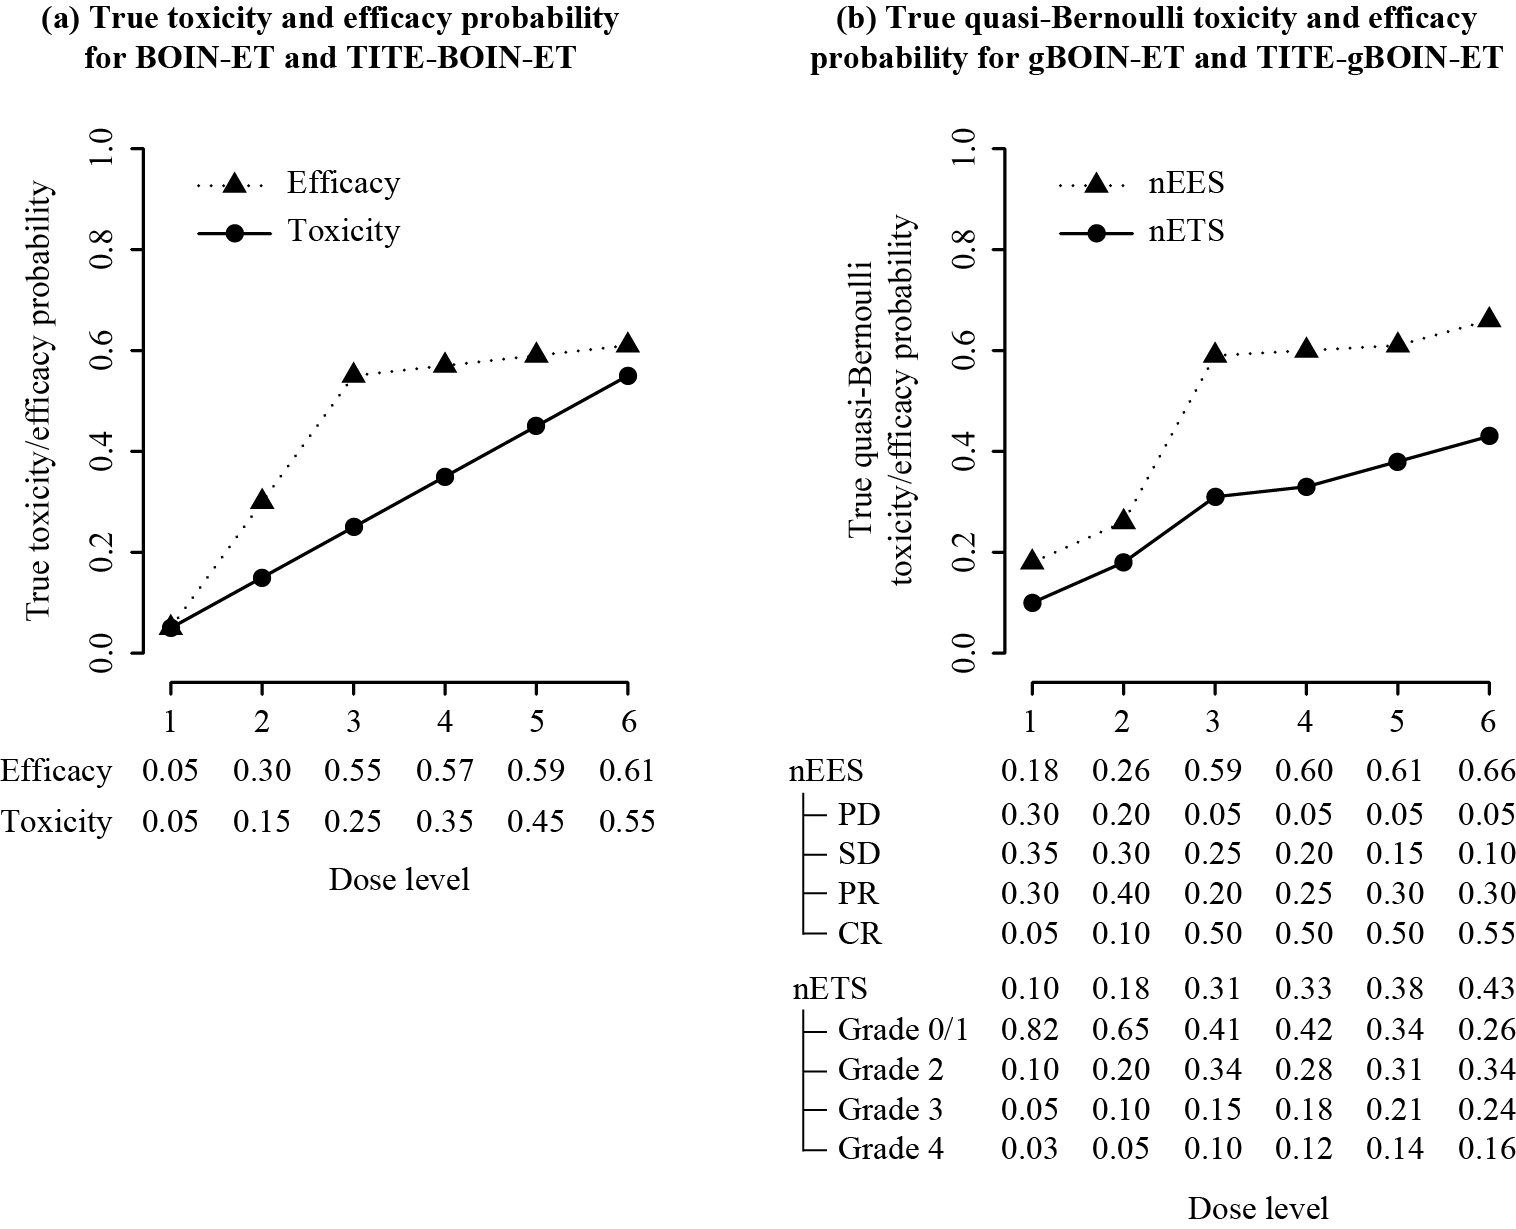
\includegraphics{figure1}
  \caption{Dose-toxicity and dose-efficacy relationship considered in simulation study.}
\end{figure}

\subsection{BOIN-ET}
The \code{boinet()} function supports the conduct of simulation studies for the BOIN-ET design and returns a list of the summary results. The usage of the \code{boinet()} function is as follows:
\begin{example}
boinet(
  n.dose, start.dose, size.cohort, n.cohort,
  toxprob, effprob,
  phi=0.3, phi1=phi*0.1, phi2=phi*1.4, delta=0.6, delta1=delta*0.6,
  alpha.T1=0.5, alpha.E1=0.5, tau.T, tau.E,
  te.corr=0.2, gen.event.time="weibull",
  accrual, gen.enroll.time="uniform",
  stopping.npts=size.cohort*n.cohort,
  stopping.prob.T=0.95, stopping.prob.E=0.99,
  estpt.method="obs.prob", obd.method="max.effprob",
  w1=0.33, w2=1.09,
  plow.ast=phi1, pupp.ast=phi2, qlow.ast=delta1/2, qupp.ast=delta,
  psi00=40, psi11=60,
  n.sim=1000, seed.sim=100)
\end{example}
Some of the key arguments are detailed in Table 1, 2, 3, and 4 in Appendix. Here, \code{toxprob} and \code{effprob} are vectors of true toxicity and efficacy probabilities with a length equal to the number of dose levels investigated.

We considered a scenario of the true toxicity and efficacy probabilities as given in Figure 1(a):
\begin{example}
> toxprob <- c(0.05,0.15,0.25,0.35,0.45,0.55)
> effprob <- c(0.05,0.30,0.55,0.57,0.59,0.61)
\end{example}
and used (i) the observed efficacy probability for the efficacy probability estimation and (ii) the highest estimated efficacy probability as the measure to select the OBD:
\begin{example}
> estpt.method <- "obs.prob"
> obd.method   <- "max.effprob"
\end{example}
Then, the \code{boinet()} is implemented with the previously specified arguments:
\begin{example}
> boinet(
+   n.dose=n.dose, start.dose=start.dose,
+   size.cohort=size.cohort, n.cohort=n.cohort,
+   toxprob=toxprob, effprob=effprob,
+   phi=phi, delta=delta,
+   tau.T=tau.T, tau.E=tau.E, accrual=accrual,
+   estpt.method=estpt.method, obd.method=obd.method)
\end{example}
and returns the following output:
\begin{example}
Simulation results:

                 Dose1  Dose2  Dose3  Dose4  Dose5  Dose6
Toxicity prob.    0.05   0.15   0.25   0.35   0.45   0.55
Efficacy prob.    0.05   0.30   0.55   0.57   0.59   0.61
No. Pts treated   3.40   7.00  15.90   7.00   2.00   0.60
Select %          1.70  12.00  54.40  25.50   5.30   0.80

No OBD %                 0.3
Trial duration (days)  778.9

Trial design settings:

Target toxicity prob.    0.330
Target efficacy prob.    0.600
Lower toxicity boundary  0.153
Upper toxicity boundary  0.390
Lower efficacy boundary  0.480

Tox. assessment window (days)  30
Eff. assessment window (days)  45
Accrual rate (days)            10

Efficacy prob. estimation: obs.prob

OBD selection: max.effprob
\end{example}
The simulation results include the number or the percentage of times that each dose level was selected as OBD (\code{Select \%}), the average number of patients who were treated at each dose level (\code{No. Pts treated}), the percentage of times that the study was terminated (\code{Stop \%}), and the expected study duration (\code{Trial duration (days)}). The trial design settings, such as the lower and upper toxicity/efficacy boundaries used for the dose-escalation, are also displayed. The average number of patients treated at Dose 3 was 15.90, and Dose 3 was selected as an OBD in 54.40\% of the simulated trials, on average. The OBD was not selected in 0.3\% of the simulated trials, on average. The trial duration was an average of 778.9 days.

\subsection{TITE-BOIN-ET}
The \code{tite.boinet()} function supports the conduct of simulation studies for the TITE-BOIN-ET design and returns a list of the summary results. The usage of the \code{tite.boinet()} function is as follows:
\begin{example}
tite.boinet(
  n.dose, start.dose, size.cohort, n.cohort,
  toxprob, effprob,
  phi=0.3, phi1=phi*0.1, phi2=phi*1.4, delta=0.6, delta1=delta*0.6,
  alpha.T1=0.5, alpha.E1=0.5, tau.T, tau.E,
  te.corr=0.2, gen.event.time="weibull",
  accrual, gen.enroll.time="uniform",
  stopping.npts=size.cohort*n.cohort,
  stopping.prob.T=0.95, stopping.prob.E=0.99,
  estpt.method="obs.prob", obd.method="max.effprob",
  w1= 0.33, w2=1.09,
  plow.ast=phi1, pupp.ast=phi2, qlow.ast=delta1/2, qupp.ast=delta,
  psi00=40, psi11=60,
  n.sim=1000, seed.sim=100)
\end{example}
Some of the key arguments are detailed in Table 1, 2, 3, and 4 in Appendix. It should be noted that the TITE-BOIN-ET design has a suspension rule which holds off the decision on dose allocation (i.e., patient enrollment to the next cohort) until adequate information is collected, where the dose allocation is allowed only if more than 50\% of patients have finished the assessment at the current dose level.

We considered a scenario of the true toxicity and efficacy probabilities as given in Figure 1(a):
\begin{example}
> toxprob <- c(0.05,0.15,0.25,0.35,0.45,0.55)
> effprob <- c(0.05,0.30,0.55,0.57,0.59,0.61)
\end{example}
and used (i) the observed efficacy probability for the efficacy probability estimation and (ii) the highest estimated efficacy probability as the measure to select the OBD:
\begin{example}
> estpt.method <- "obs.prob"
> obd.method   <- "max.effprob"
\end{example}
Then, the \code{tite.boinet()} is implemented with the previously specified arguments:
\begin{example}
> tite.boinet(
+   n.dose=n.dose, start.dose=start.dose,
+   size.cohort=size.cohort, n.cohort=n.cohort,
+   toxprob=toxprob, effprob=effprob,
+   phi=phi, delta=delta,
+   tau.T=tau.T, tau.E=tau.E, accrual=accrual,
+   estpt.method=estpt.method, obd.method=obd.method)
\end{example}
and returns the following output:
\begin{example}
Simulation results:

                 Dose1  Dose2  Dose3  Dose4  Dose5  Dose6
Toxicity prob.    0.05   0.15   0.25   0.35   0.45   0.55
Efficacy prob.    0.05   0.30   0.55   0.57   0.59   0.61
No. Pts treated   3.60   6.40  14.60   7.40   3.00   0.90
Select %          1.80  12.90  55.10  22.50   6.20   1.00

No OBD %                 0.5
Trial duration (days)  476.5

Trial design settings:

Target toxicity prob.    0.330
Target efficacy prob.    0.600
Lower toxicity boundary  0.153
Upper toxicity boundary  0.390
Lower efficacy boundary  0.480

Tox. assessment window (days)  30
Eff. assessment window (days)  45
Accrual rate (days)            10

Efficacy prob. estimation: obs.prob

OBD selection: max.effprob
\end{example}
The average number of patients treated at Dose 3 was 14.60, and Dose 3 was selected as an OBD in 55.10\% of the simulated trials, on average. The OBD was not selected in 0.5\% of the simulated trials, on average. The trial duration was an average of 476.5 days.

\subsection{gBOIN-ET}
The \code{gboinet()} function supports the conduct of simulation studies for the gBOIN-ET design and returns a list of the summary results. The usage of the \code{gboinet()} function is as follows:
\begin{example}
gboinet(
  n.dose, start.dose, size.cohort, n.cohort,
  toxprob, effprob, sev.weight, res.weight,
  phi, phi1=phi*0.1, phi2=phi*1.4, delta, delta1=delta*0.6,
  alpha.T1=0.5, alpha.E1=0.5, tau.T, tau.E,
  te.corr=0.2, gen.event.time="weibull",
  accrual, gen.enroll.time="uniform",
  stopping.npts=size.cohort*n.cohort,
  stopping.prob.T=0.95, stopping.prob.E=0.99,
  estpt.method="obs.prob", obd.method="max.effprob",
  w1=0.33, w2=1.09,
  plow.ast=phi1, pupp.ast=phi2, qlow.ast=delta1/2, qupp.ast=delta,
  psi00=40, psi11=60,
  n.sim=1000, seed.sim=100)
\end{example}
Some of the key arguments are detailed in Table 1, 2, 3, and 4 in Appendix. Here, \code{toxprob} and \code{effprob} are matrices of true quasi-Bernoulli toxicity and efficacy probabilities with a row length equal to the number of outcome categories and a column length equal to the number of dose levels investigated. \code{sev.weight} and \code{res.weight} are weights assigned to toxicity and efficacy outcome categories respectively. For example, considering the ETS and EES, we can use \code{sev.weight=c(0.00,0.50,1.00,1.50)} for grade 0/1, 2, 3, and 4 toxicity and \code{res.weight=c(0.00,0.25,1.00,3.00)} for PD, SD, PR, and CR efficacy response, respectively

We considered a scenario of the true quasi-Bernoulli toxicity and efficacy probabilities as given in Figure 1(b):
\begin{example}
> toxprob <- rbind(c(0.82,0.65,0.41,0.42,0.34,0.26),
+                  c(0.10,0.20,0.34,0.28,0.31,0.34),
+                  c(0.05,0.10,0.15,0.18,0.21,0.24),
+                  c(0.03,0.05,0.10,0.12,0.14,0.16))
> 
> effprob <- rbind(c(0.30,0.20,0.05,0.05,0.05,0.05),
+                  c(0.35,0.30,0.25,0.20,0.15,0.10),
+                  c(0.30,0.40,0.20,0.25,0.30,0.30),
+                  c(0.05,0.10,0.50,0.50,0.50,0.55))
\end{example}
The weights assigned to toxicity and efficacy outcome categories were given by:
\begin{example}
> sev.weight <- c(0.00,0.50,1.00,1.50)
> res.weight <- c(0.00,0.25,1.00,3.00)
\end{example}
and we used (i) the observed efficacy probability for the efficacy probability estimation and (ii) the highest estimated efficacy probability as the measure to select the OBD:
\begin{example}
> estpt.method <- "obs.prob"
> obd.method   <- "max.effprob"
\end{example}
Then, the \code{gboinet()} is implemented with the previously specified arguments:
\begin{example}
> gboinet(
+   n.dose=n.dose, start.dose=start.dose,
+   size.cohort=size.cohort, n.cohort=n.cohort,
+   toxprob=toxprob, effprob=effprob,
+   sev.weight=sev.weight, res.weight=res.weight,
+   phi=phi, delta=delta,
+   tau.T=tau.T, tau.E=tau.E, accrual=accrual,
+   estpt.method=estpt.method, obd.method=obd.method)
\end{example}
and returns the following output:
\begin{example}
Simulation results:

                 Dose1  Dose2  Dose3  Dose4  Dose5  Dose6
Tox.cat1          0.82   0.65   0.41   0.42   0.34   0.26
Tox.cat2          0.10   0.20   0.34   0.28   0.31   0.34
Tox.cat3          0.05   0.10   0.15   0.18   0.21   0.24
Tox.cat4          0.03   0.05   0.10   0.12   0.14   0.16
nETS              0.10   0.18   0.31   0.33   0.38   0.43
Eff.cat1          0.30   0.20   0.05   0.05   0.05   0.05
Eff.cat2          0.35   0.30   0.25   0.20   0.15   0.10
Eff.cat3          0.30   0.40   0.20   0.25   0.30   0.30
Eff.cat4          0.05   0.10   0.50   0.50   0.50   0.55
nEES              0.18   0.26   0.59   0.60   0.61   0.66
No. Pts treated   3.80   7.20  17.60   5.40   1.70   0.30
Select %          2.90   8.20  63.10  19.50   5.50   0.70

No OBD %                 0.1
Trial duration (days)  780.1

Trial design settings:

Target toxicity prob.    0.330
Target efficacy prob.    0.600
Lower toxicity boundary  0.153
Upper toxicity boundary  0.390
Lower efficacy boundary  0.480

Tox. assessment window (days)  30
Eff. assessment window (days)  45
Accrual rate (days)            10

Efficacy prob. estimation: obs.prob

OBD selection: max.effprob
\end{example}
The average number of patients treated at Dose 3 was 17.60, and Dose 3 was selected as an OBD in 63.10\% of the simulated trials, on average. The OBD was not selected in 0.1\% of the simulated trials, on average. The trial duration was an average of 780.1 days.

\subsection{TITE-gBOIN-ET}
The \code{tite.gboinet()} function supports the conduct of simulation studies for the gBOIN-ET design and returns a list of the summary results. The usage of the \code{tite.gboinet()} function is as follows:
\begin{example}
tite.gboinet(
  n.dose, start.dose, size.cohort, n.cohort,
  toxprob, effprob, sev.weight, res.weight,
  phi, phi1=phi*0.1, phi2=phi*1.4, delta, delta1=delta*0.6,
  alpha.T1=0.5, alpha.E1=0.5, tau.T, tau.E,
  te.corr=0.2, gen.event.time="weibull",
  accrual, gen.enroll.time="uniform",
  stopping.npts=size.cohort*n.cohort,
  stopping.prob.T=0.95, stopping.prob.E=0.99,
  estpt.method="obs.prob", obd.method="max.effprob",
  w1=0.33, w2=1.09,
  plow.ast=phi1, pupp.ast=phi2, qlow.ast=delta1/2, qupp.ast=delta,
  psi00=40, psi11=60,
  n.sim=1000, seed.sim=100)
\end{example}
Some of the key arguments are detailed in Table 1, 2, 3, and 4 in Appendix. It should be noted that the TITE-gBOIN-ET design has a suspension rule which holds off the decision on dose allocation (i.e., patient enrollment to the next cohort) until adequate information is collected, where the dose allocation is allowed only if more than 50\% of patients have finished the assessment at the current dose level.

We considered a scenario of the true quasi-Bernoulli toxicity and efficacy probabilities as given in Figure 1(b):
\begin{example}
> toxprob <- rbind(c(0.82,0.65,0.41,0.42,0.34,0.26),
+                  c(0.10,0.20,0.34,0.28,0.31,0.34),
+                  c(0.05,0.10,0.15,0.18,0.21,0.24),
+                  c(0.03,0.05,0.10,0.12,0.14,0.16))
> 
> effprob <- rbind(c(0.30,0.20,0.05,0.05,0.05,0.05),
+                  c(0.35,0.30,0.25,0.20,0.15,0.10),
+                  c(0.30,0.40,0.20,0.25,0.30,0.30),
+                  c(0.05,0.10,0.50,0.50,0.50,0.55))
\end{example}
The weights assigned to toxicity and efficacy outcome categories were given by:
\begin{example}
> sev.weight <- c(0.00,0.50,1.00,1.50)
> res.weight <- c(0.00,0.25,1.00,3.00)
\end{example}
and we used (i) the observed efficacy probability for the efficacy probability estimation and (ii) the highest estimated efficacy probability as the measure to select the OBD:
\begin{example}
> estpt.method <- "obs.prob"
> obd.method   <- "max.effprob"
\end{example}
Then, the \code{tite.gboinet()} is implemented with the previously specified arguments:
\begin{example}
> tite.gboinet(
+   n.dose=n.dose, start.dose=start.dose,
+   size.cohort=size.cohort, n.cohort=n.cohort,
+   toxprob=toxprob, effprob=effprob,
+   sev.weight=sev.weight, res.weight=res.weight,
+   phi=phi, delta=delta,
+   tau.T=tau.T, tau.E=tau.E, accrual=accrual,
+   estpt.method=estpt.method, obd.method=obd.method)
\end{example}
and returns the following output:
\begin{example}
Simulation results:

                 Dose1  Dose2  Dose3  Dose4  Dose5  Dose6
Tox.cat1          0.82   0.65   0.41   0.42   0.34   0.26
Tox.cat2          0.10   0.20   0.34   0.28   0.31   0.34
Tox.cat3          0.05   0.10   0.15   0.18   0.21   0.24
Tox.cat4          0.03   0.05   0.10   0.12   0.14   0.16
nETS              0.10   0.18   0.31   0.33   0.38   0.43
Eff.cat1          0.30   0.20   0.05   0.05   0.05   0.05
Eff.cat2          0.35   0.30   0.25   0.20   0.15   0.10
Eff.cat3          0.30   0.40   0.20   0.25   0.30   0.30
Eff.cat4          0.05   0.10   0.50   0.50   0.50   0.55
nEES              0.18   0.26   0.59   0.60   0.61   0.66
No. Pts treated   3.90   7.20  15.70   6.20   2.40   0.60
Select %          3.00   8.10  61.00  20.70   5.90   1.20

No OBD %                 0.1
Trial duration (days)  441.0

Trial design settings:

Target toxicity prob.    0.330
Target efficacy prob.    0.600
Lower toxicity boundary  0.153
Upper toxicity boundary  0.390
Lower efficacy boundary  0.480

Tox. assessment window (days)  30
Eff. assessment window (days)  45
Accrual rate (days)            10

Efficacy prob. estimation: obs.prob

OBD selection: max.effprob
\end{example}
The average number of patients treated at Dose 3 was 15.70, and Dose 3 was selected as an OBD in 61.00\% of the simulated trials, on average. The OBD was not selected in 0.1\% of the simulated trials, on average. The trial duration was an average of 441.0 days.

\section{Summary}
The concept of OBD is now widely accepted as an alternative to MTD in oncology dose-finding trials, and the BOIN-ET design family is simple and flexible enough to establish the OBD while accounting for toxicity and efficacy in the framework of dose-finding. The \CRANpkg{boinet} package has been developed to support the conduct of simulation studies to assess operating characteristics of BOIN-ET, TITE-BOIN-ET, gBOIN-ET, and TITE-gBOIN-ET designs. Users can choose design parameters in flexible and straightforward ways depending on their own application, and several options regarding methods to estimate the efficacy probability and measures to select the OBD are applicable. The package would assist practitioners in efficiently assessing the design features of their studies.

\bibliography{RJ-boinet}

\address{Yusuke Yamaguchi\\
  Quantitative Sciences and Evidence Generation, Astellas Pharma Global Development, Inc.\\
  2375 Waterview Drive, Northbrook, Illinois 60062\\
  United States\\
  \email{yusuke-yamaguchi@astellas.com}}

\address{Kentaro Takeda\\
  Quantitative Sciences and Evidence Generation, Astellas Pharma Global Development, Inc.\\
  2375 Waterview Drive, Northbrook, Illinois 60062\\
  United States\\
  \email{kentaro.takeda@astellas.com}}

\address{Kazushi Maruo\\
  Department of Biostatistics, Faculty of Medicine, University of Tsukuba\\
  1-1-1, Tennodai, Tsukuba, Ibaraki 305-8577\\
  Japan\\
  \email{kazushi.maruo@gmail.com}}

~\\
\newpage

\section{Appendix: Key arguments used in \texorpdfstring{\code{boinet()}, \code{tite.boinet()}, \code{gboinet()}, and \code{tite.gboinet()}}{boinet(), tite.boinet(), gboinet(), and tite.gboinet()} function}

\begin{table}[!ht]
\begin{tabular}{p{2.6cm}p{10.5cm}}
\hline
Argument & Description\\
\hline
\code{phi} & Numeric value between 0 and 1 specifying the target (quasi-Bernoulli) toxicity probability. Represents the maximum acceptable toxicity rate. Default is 0.3 (30\%).\\
\code{phi1} & Numeric value specifying the highest (quasi-Bernoulli) toxicity probability that is deemed sub-therapeutic such that dose-escalation should be pursued. Default is phi*0.1.\\
\code{phi2} & Numeric value specifying the lowest (quasi-Bernoulli) toxicity probability that is deemed overly toxic such that dose de-escalation is needed. Default is phi*1.4.\\
\code{delta} & Numeric value between 0 and 1 specifying the target (quasi-Bernoulli) efficacy probability. Represents the desired minimum efficacy rate. Default is 0.6 (60\%).\\
\code{delta1} & Numeric value specifying the minimum probability deemed efficacious such that the dose levels with efficacy < delta1 are considered sub-therapeutic. Default is delta*0.6.\\
\hline
\end{tabular}
\centering
\caption{Arguments regarding target (quasi-Bernoulli) toxicity and efficacy probability.}
\end{table}

\begin{table}[!ht]
\begin{tabular}{p{2.6cm}p{10.5cm}}
\hline
Argument & Description\\
\hline
\code{alpha.T1} & Numeric value specifying the probability that a (quasi-Bernoulli) toxicity outcome occurs in the late half of the toxicity assessment window. Used for event time generation. Default is 0.5.\\
\code{alpha.E1} & Numeric value specifying the probability that a (quasi-Bernoulli) efficacy outcome occurs in the late half of the efficacy assessment window. Used for event time generation. Default is 0.5.\\
\code{te.corr} & Numeric value between -1 and 1 specifying the correlation between toxicity and efficacy, specified as Gaussian copula parameter. Default is 0.2 (weak positive correlation).\\
\code{gen.event.time} & Character string specifying the distribution for generating event times. Options are "weibull" (default) or "uniform". A bivariate Gaussian copula model is used to jointly generate the time to first toxicity and efficacy outcome, where the marginal distributions are set to Weibull distribution when \code{gen.event.time="weibull"}, and uniform distribution when \code{gen.event.time="uniform"}.\\
\code{gen.enroll.time} & Character string specifying the distribution for enrollment times. Options are "uniform" (default) or "exponential". Uniform distribution is used when \code{gen.enroll.time="uniform"}, and exponential distribution is used when \code{gen.enroll.time="exponential"}.\\
\hline
\end{tabular}
\centering
\caption{Arguments regarding data generation.}
\end{table}

\begin{table}[!ht]
\begin{tabular}{p{2.6cm}p{10.5cm}}
\hline
Argument & Description\\
\hline
\code{stopping.npts} & Integer specifying the maximum number of patients per dose for early study termination. If the number of patients at the current dose reaches this criterion, the study stops the enrollment and is terminated. Default is size.cohort*n.cohort.\\
\code{stopping.prob.T} & Numeric value between 0 and 1 specifying the early study termination threshold for toxicity. If P(toxicity > phi) > stopping.prob.T, the dose levels are eliminated from the investigation. Default is 0.95.\\
\code{stopping.prob.E} & Numeric value between 0 and 1 specifying the early study termination threshold for efficacy. If P(efficacy < delta1) > stopping.prob.E, the dose levels are eliminated from the investigation. Default is 0.99.\\
\hline
\end{tabular}
\centering
\caption{Arguments regarding early study termination criteria.}
\end{table}

\begin{table}[!ht]
\begin{tabular}{p{2.6cm}p{10.5cm}}
\hline
Argument & Description\\
\hline
\code{estpt.method} & Character string specifying the method for estimating efficacy probabilities. Options: "obs.prob" (observed efficacy probabilities/rates), "fp.logistic" (fractional polynomial), or "multi.iso" (model averaging of multiple unimodal isotonic regression). Default is "obs.prob".\\
\code{obd.method} & Character string specifying the method for OBD selection. Options: "utility.weighted", "utility.truncated.linear", "utility.scoring", or "max.effprob" (default).\\
\hline
\code{w1} & Numeric value specifying the weight for toxicity-efficacy trade-off in "utility.weighted" method. Default is 0.33.\\
\code{w2} & Numeric value specifying the penalty weight for toxic doses in "utility.weighted" method. Default is 1.09.\\
\code{plow.ast} & Numeric value specifying the lower toxicity threshold for "utility.truncated.linear" method. Default is phi1.\\
\code{pupp.ast} & Numeric value specifying the upper toxicity threshold for "utility.truncated.linear" method. Default is phi2.\\
\code{qlow.ast} & Numeric value specifying the lower efficacy threshold for "utility.truncated.linear" method. Default is delta1/2.\\
\code{qupp.ast} & Numeric value specifying the upper efficacy threshold for "utility.truncated.linear" method. Default is delta.\\
\code{psi00} & Numeric value specifying the utility score for (toxicity=no, efficacy=no) in "utility.scoring" method. Default is 40.\\
\code{psi11} & Numeric value specifying the utility score for (toxicity=yes, efficacy=yes) in "utility.scoring" method. Default is 60.\\
\hline
\end{tabular}
\centering
\caption{Arguments regarding optimal biological dose (OBD) selection.}
\end{table}
